% !TeX root = ../../../thoulon_phd_defense_2025.tex


\documentclass{standalone}
%%% Preamble Requirements %%%
\usepackage{geometry}
\usepackage{amsfonts}
\usepackage{amsmath}
\usepackage{amssymb}
\usepackage{tikz}

% Optional packages such as sfmath set through python interface
\usepackage{sfmath}

\usetikzlibrary{arrows,chains,positioning,scopes,shapes.geometric,shapes.misc,shadows,matrix}

%%% End Preamble Requirements %%%

\begin{document}

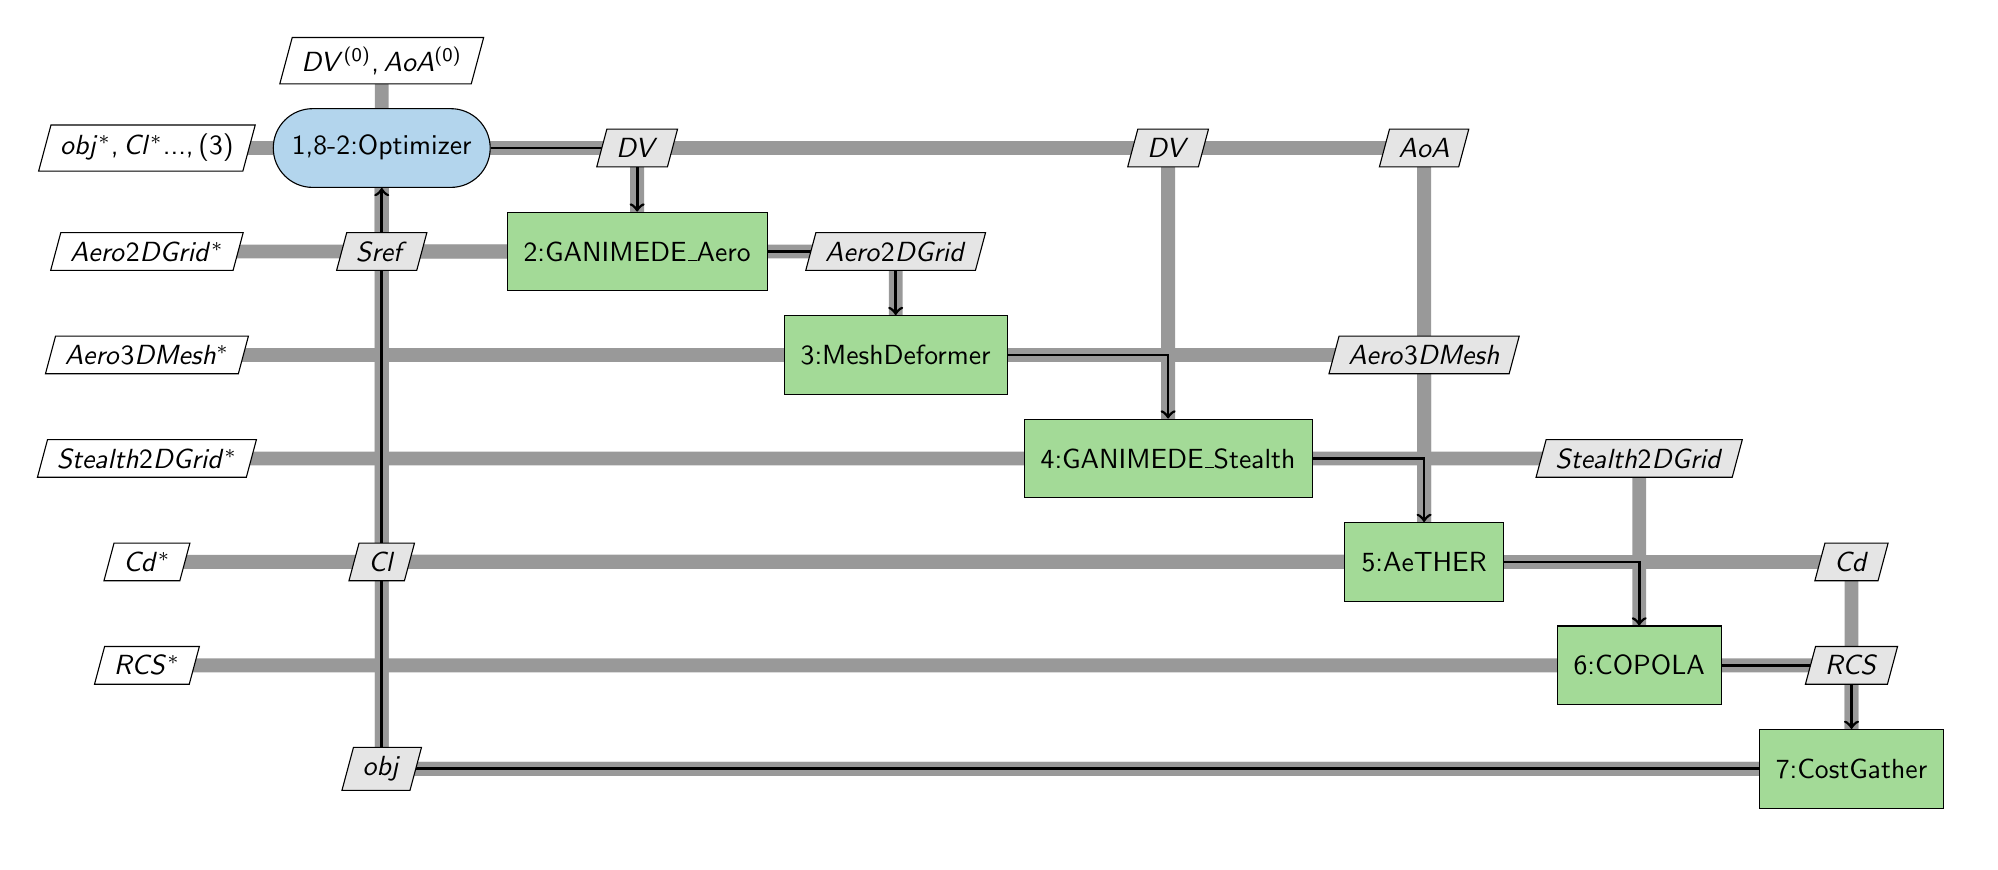
\begin{tikzpicture}
% Define all the styles used to produce XDSMs for MDO

% Tableau 20 color palette, taken from
% https://jrnold.github.io/ggthemes/reference/tableau_color_pal.html
% we use the lighter variants here with 80% opacity
% Blue
\definecolor{red}{HTML}{A0CBE8}
% Orange
\definecolor{orange}{HTML}{FFBE7D}
% Cyan
\definecolor{cyan}{HTML}{86BCB6}
% Green
\definecolor{green}{HTML}{8CD17D}
% Yellow
\definecolor{yellow}{HTML}{F1CE63}
% Salmon
\definecolor{salmon}{HTML}{FF9D9A}

\tikzstyle{every node}=[font=\sffamily,align=center]

\newcommand{\fillOpacity}{80}%

% Component shapes
\newcommand{\compShape}{rectangle}%
\newcommand{\groupShape}{chamfered rectangle}%
\newcommand{\procShape}{rounded rectangle}%

% Colors
\newcommand{\explicitColor}{green}%
\newcommand{\implicitColor}{salmon}%
\newcommand{\optimizationColor}{red}% also used by DOE

% Component types
\tikzstyle{Optimization} = [\procShape,draw,fill=\optimizationColor!\fillOpacity,inner sep=6pt,minimum height=1cm,text badly centered]
\tikzstyle{MDA} = [\procShape,draw,fill=orange!\fillOpacity,inner sep=6pt,minimum height=1cm,text badly centered]
\tikzstyle{DOE} = [\procShape,draw,fill=\optimizationColor!\fillOpacity,inner sep=6pt,minimum height=1cm,text badly centered]
\tikzstyle{SubOptimization} = [\groupShape,draw,fill=\optimizationColor!\fillOpacity,inner sep=6pt,minimum height=1cm,text badly centered]
\tikzstyle{Group} = [\groupShape,draw,fill=\explicitColor!\fillOpacity,inner sep=6pt,minimum height=1cm,text badly centered]
\tikzstyle{ImplicitGroup} = [\groupShape,draw,fill=\implicitColor!\fillOpacity,inner sep=6pt,minimum height=1cm,text badly centered]
\tikzstyle{Function} = [\compShape,draw,fill=\explicitColor!\fillOpacity,inner sep=6pt,minimum height=1cm,text badly centered]
\tikzstyle{ImplicitFunction} = [\compShape,draw,fill=\implicitColor!\fillOpacity,inner sep=6pt,minimum height=1cm,text badly centered]
\tikzstyle{Metamodel} = [\compShape,draw,fill=yellow!\fillOpacity,inner sep=6pt,minimum height=1cm,text badly centered]

%% A simple command to give the repeated structure look for components and data
\tikzstyle{stack} = [double copy shadow={shadow xshift=.75ex, shadow yshift=-.75ex}]
%% A simple command to fade components and data, e.g. demonstrating a sequence of steps in an animation
\tikzstyle{faded} = [draw=black!10,fill=white,text opacity=0.2]

%% Simple fading commands for the lines
\tikzstyle{fadeddata} = [color=black!20]
\tikzstyle{fadedprocess} = [color=black!50]

% Data types
\newcommand{\dataRightAngle}{105}%
\newcommand{\dataLeftAngle}{75}%

\tikzstyle{DataInter} = [trapezium,trapezium left angle=\dataLeftAngle,trapezium right angle=\dataRightAngle,draw,fill=black!10]
\tikzstyle{DataIO} = [trapezium,trapezium left angle=\dataLeftAngle,trapezium right angle=\dataRightAngle,draw,fill=white]

% Edges
\tikzstyle{DataLine} = [color=black!40,line width=5pt,line cap=rect]
\tikzstyle{ProcessHV} = [-,line width=1pt,to path={-| (\tikztotarget)}]
\tikzstyle{ProcessHVA} = [->,line width=1pt,to path={-| (\tikztotarget)}]
\tikzstyle{ProcessTip} = [-,line width=1pt]
\tikzstyle{ProcessTipA} = [->, line width=1pt]
\tikzstyle{FadedProcessHV} = [-,line width=1pt,to path={-| (\tikztotarget)},color=black!30]
\tikzstyle{FadedProcessHVA} = [->,line width=1pt,to path={-| (\tikztotarget)},color=black!30]
\tikzstyle{FadedProcessTip} = [-,line width=1pt,color=black!30]
\tikzstyle{FadedProcessTipA} = [->, line width=1pt,color=black!30]

% Matrix options
\tikzstyle{MatrixSetup} = [row sep=3mm, column sep=2mm]

% Declare a background layer for showing node connections
\pgfdeclarelayer{data}
\pgfdeclarelayer{process}
\pgfsetlayers{data,process,main}

% A new command to split the component text over multiple lines

\newcommand{\MultilineComponent}[2]
{
	\begin{minipage}{#1}
	\begin{center}
		#2
	\end{center}
	\end{minipage}
}

\newcommand{\TwolineComponent}[3]
{
	\begin{minipage}{#1}
	\begin{center}
		#2 \linebreak #3
	\end{center}
	\end{minipage}
}

\newcommand{\ThreelineComponent}[4]
{
	\begin{minipage}{#1}
	\begin{center}
		#2 \linebreak #3 \linebreak #4
	\end{center}
	\end{minipage}
}

% A new command to split the component text over multiple columns
\newcommand{\MultiColumnComponent}[5]
{
	\begin{minipage}{#1}
	\begin{center}
	#2 \linebreak #3
	\end{center}
	\begin{minipage}{0.49\textwidth}
	\begin{center}
	#4
	\end{center}
	\end{minipage}
	\begin{minipage}{0.49\textwidth}
	\begin{center}
	#5
	\end{center}
	\end{minipage}
	\end{minipage}
}

\def\arraystretch{1.3}%
%
\matrix[MatrixSetup]{
%Row 0
&
\node [DataIO] (output_Opt) {$DV^{(0)},  AoA^{(0)}$};&
&
&
&
&
&
&
\\
%Row 1
\node [DataIO] (left_output_Opt) {$obj^*,  Cl^*..., (3)$};&
\node [Optimization] (Opt) {$\text{1,8-2:Optimizer}$};&
\node [DataInter] (Opt-Dis1) {$DV$};&
&
\node [DataInter] (Opt-Dis3) {$DV$};&
\node [DataInter] (Opt-Dis4) {$AoA$};&
&
&
\\
%Row 2
\node [DataIO] (left_output_Dis1) {$Aero2DGrid^*$};&
\node [DataInter] (Dis1-Opt) {$Sref$};&
\node [Function] (Dis1) {$\text{2:GANIMEDE\_Aero}$};&
\node [DataInter] (Dis1-Dis2) {$Aero2DGrid$};&
&
&
&
&
\\
%Row 3
\node [DataIO] (left_output_Dis2) {$Aero3DMesh^*$};&
&
&
\node [Function] (Dis2) {$\text{3:MeshDeformer}$};&
&
\node [DataInter] (Dis2-Dis4) {$Aero3DMesh$};&
&
&
\\
%Row 4
\node [DataIO] (left_output_Dis3) {$Stealth2DGrid^*$};&
&
&
&
\node [Function] (Dis3) {$\text{4:GANIMEDE\_Stealth}$};&
&
\node [DataInter] (Dis3-Dis5) {$Stealth2DGrid$};&
&
\\
%Row 5
\node [DataIO] (left_output_Dis4) {$Cd^*$};&
\node [DataInter] (Dis4-Opt) {$Cl$};&
&
&
&
\node [Function] (Dis4) {$\text{5:AeTHER}$};&
&
\node [DataInter] (Dis4-Dis6) {$Cd$};&
\\
%Row 6
\node [DataIO] (left_output_Dis5) {$RCS^*$};&
&
&
&
&
&
\node [Function] (Dis5) {$\text{6:COPOLA}$};&
\node [DataInter] (Dis5-Dis6) {$RCS$};&
\\
%Row 7
&
\node [DataInter] (Dis6-Opt) {$obj$};&
&
&
&
&
&
\node [Function] (Dis6) {$\text{7:CostGather}$};&
\\
%Row 8
&
&
&
&
&
&
&
&
\\
};

% XDSM process chains
{ [start chain=process]
\begin{pgfonlayer}{process} 
\chainin (Opt);
\chainin (Dis1) [join=by ProcessHVA];
\end{pgfonlayer}
}{ [start chain=process]
 \begin{pgfonlayer}{process} 
\chainin (Dis1);
\chainin (Dis2) [join=by ProcessHVA];
\end{pgfonlayer}
}{ [start chain=process]
 \begin{pgfonlayer}{process} 
\chainin (Dis2);
\chainin (Dis3) [join=by ProcessHVA];
\end{pgfonlayer}
}{ [start chain=process]
 \begin{pgfonlayer}{process} 
\chainin (Dis3);
\chainin (Dis4) [join=by ProcessHVA];
\end{pgfonlayer}
}{ [start chain=process]
 \begin{pgfonlayer}{process} 
\chainin (Dis4);
\chainin (Dis5) [join=by ProcessHVA];
\end{pgfonlayer}
}{ [start chain=process]
 \begin{pgfonlayer}{process} 
\chainin (Dis5);
\chainin (Dis6) [join=by ProcessHVA];
\end{pgfonlayer}
}{ [start chain=process]
 \begin{pgfonlayer}{process} 
\chainin (Dis6);
\chainin (Opt) [join=by ProcessHVA];
\end{pgfonlayer}
}

\begin{pgfonlayer}{data}
\path
% Horizontal edges
(Opt) edge [DataLine] (Opt-Dis1)
(Dis1) edge [DataLine] (Dis1-Opt)
(Opt) edge [DataLine] (Opt-Dis3)
(Opt) edge [DataLine] (Opt-Dis4)
(Dis4) edge [DataLine] (Dis4-Opt)
(Dis6) edge [DataLine] (Dis6-Opt)
(Dis1) edge [DataLine] (Dis1-Opt)
(Dis4) edge [DataLine] (Dis4-Opt)
(Dis6) edge [DataLine] (Dis6-Opt)
(Dis1) edge [DataLine] (Dis1-Dis2)
(Dis2) edge [DataLine] (Dis2-Dis4)
(Dis3) edge [DataLine] (Dis3-Dis5)
(Dis4) edge [DataLine] (Dis4-Dis6)
(Dis5) edge [DataLine] (Dis5-Dis6)
(Opt) edge [DataLine] (left_output_Opt)
(Dis1) edge [DataLine] (left_output_Dis1)
(Dis2) edge [DataLine] (left_output_Dis2)
(Dis3) edge [DataLine] (left_output_Dis3)
(Dis4) edge [DataLine] (left_output_Dis4)
(Dis5) edge [DataLine] (left_output_Dis5)
% Vertical edges
(Opt-Dis1) edge [DataLine] (Dis1)
(Dis1-Opt) edge [DataLine] (Opt)
(Opt-Dis3) edge [DataLine] (Dis3)
(Opt-Dis4) edge [DataLine] (Dis4)
(Dis4-Opt) edge [DataLine] (Opt)
(Dis6-Opt) edge [DataLine] (Opt)
(Dis1-Opt) edge [DataLine] (Opt)
(Dis4-Opt) edge [DataLine] (Opt)
(Dis6-Opt) edge [DataLine] (Opt)
(Dis1-Dis2) edge [DataLine] (Dis2)
(Dis2-Dis4) edge [DataLine] (Dis4)
(Dis3-Dis5) edge [DataLine] (Dis5)
(Dis4-Dis6) edge [DataLine] (Dis6)
(Dis5-Dis6) edge [DataLine] (Dis6)
(Opt) edge [DataLine] (output_Opt);
\end{pgfonlayer}

\end{tikzpicture}

\end{document}